\subsection{Bilan}

Notre bilan commence une comparaison de la comptabilité des solutions VPN avec les systèmes d'éxploitation les plus répandus :

\begin{figure}[H]
	\begin{center}
\begin{tabular}{l|c|c|c}
OS & Solution Windows & Solution Linux & Solution CISCO \\
\hline
Windows & Oui & Oui & Oui \\
Linux & Oui en théorie, Non en pratique & Oui & Oui \\
MAC (en théorie) & Oui & Oui & Oui \\
\end{tabular}
	\end{center}
	\caption{Compatibilité des OS}
	\label{Compatibilité_des_OS}
\end{figure}

Les solutions CISCO et OpenVPN répondent au cahier des charges en terme de compatibilité multiplate-formes. Il est à noter que nous n'avons pas pu tester nos différentes solutions sur MAC.

Afin de choisir la meilleure solution VPN, nous avons décidé de mettre des notes échelonnées de zéro (mauvais) à cinq (excellent) sur chacuns des critères que nous avons expliquer et de les regrouper dans des graphes comparatifs.

Sur chaque graphe nous trouverons les critères suivants:
\begin{itemize}
 	\item Déploiement du serveur.
 	\item Bande passante effective.
 	\item Utilisation CPU.
 	\item Coût.
 	\item Stabilité de connexion.
 	\item Déploiement du client.
	\item Niveau de sécurité.
\end{itemize}

\begin{figure}[H]
	\begin{center}
		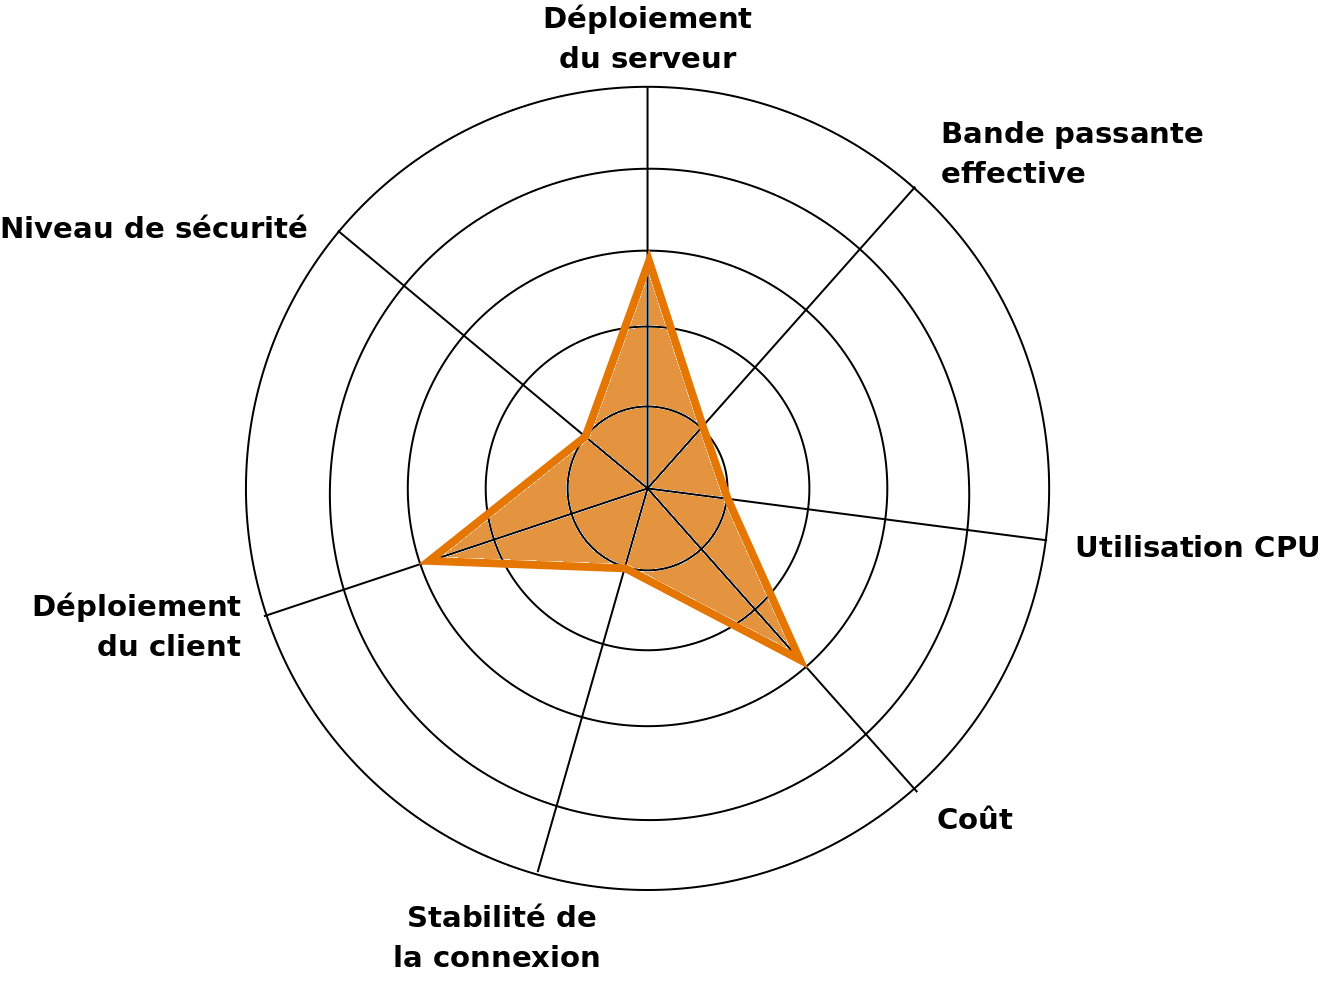
\includegraphics[width=0.6\textwidth]{partie_3/images/windows.png}\\
	\end{center}
	\caption{Bilan final de la solution Windows}
	\label{Graphe Windows}
\end{figure}

En sommant les différents critères la solution Microsoft obtient une note égale à \verb|13|

\begin{figure}[H]
	\begin{center}
		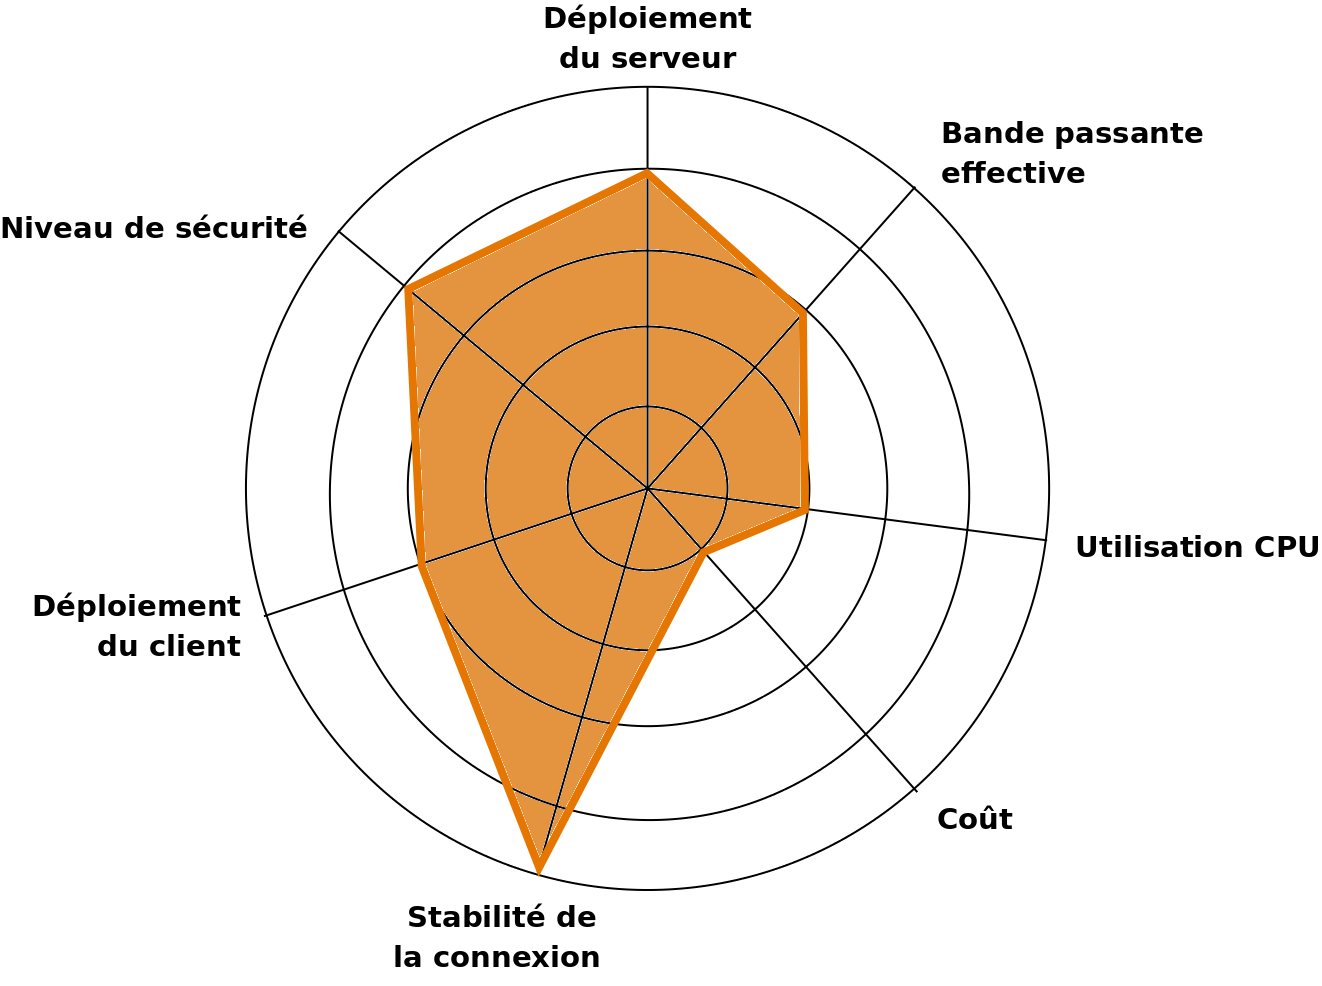
\includegraphics[width=0.6\textwidth]{partie_3/images/cisco.png}\\
	\end{center}
	\caption{Bilan final de la solution cisco}
	\label{Graphe cisco}
\end{figure}

En sommant les différents critères la solution Cisco obtient une note égale à \verb|21|

\begin{figure}[H]
	\begin{center}
		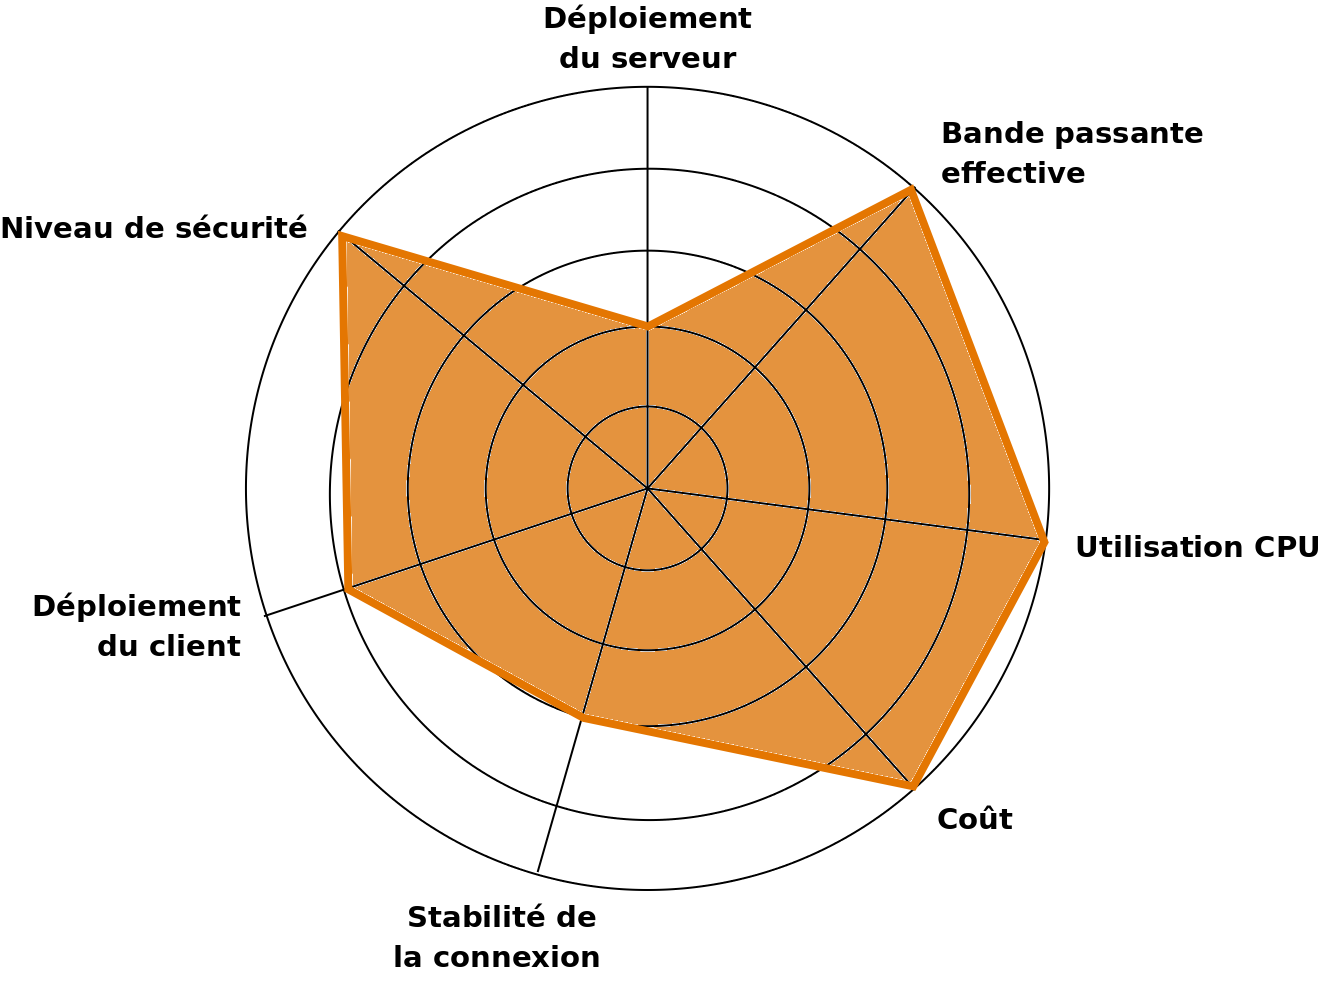
\includegraphics[width=0.7\textwidth]{partie_3/images/linux.png}\\
	\end{center}
	\caption{Bilan final de la solution Linux}
	\label{Graphe linux}
\end{figure}

En sommant les différents critères la solution Linux a une note égale à \verb|29|

~

Au vue de ces différents bilans prenant en compte l'ensemble des critères que nous avons pu aborder au cours de cette partie, nous pouvons conclure que la solution OpenVPN serait la plus adaptée à la mise en place d'un accès VPN au sein de l'ISIMA.
